\subsection{Hashing}
\begin{center}
    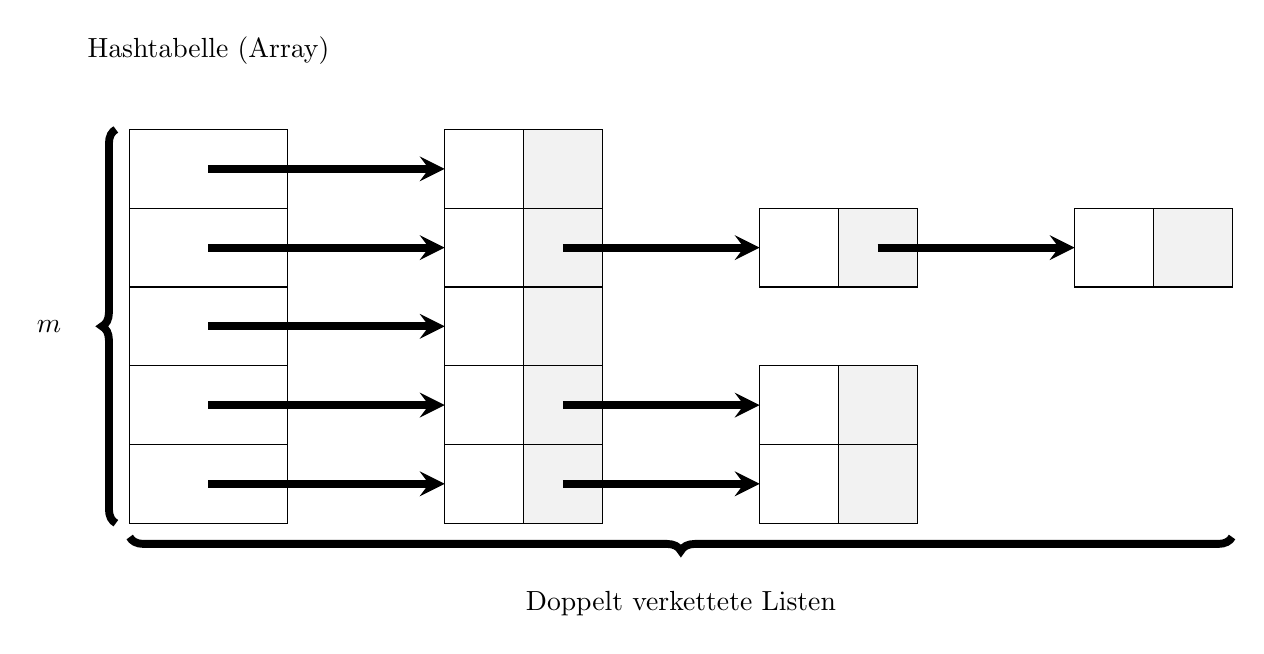
\begin{tikzpicture}
        \node (1) at (0,1) {Hashtabelle (Array)}; 
        \draw (-1, 0) rectangle ++ (2, -5);
        \foreach \x in {0,...,-4}{
            \draw[-] (-1, \x) to (1, \x);
            \draw[-stealth, thick, line width = 1mm] (0, \x - 0.5) to (3, \x - 0.5);
            
            \draw[fill=black!5!white] (3, \x) rectangle (3+2, \x-1);
            \draw[fill=white] (3, \x) rectangle (3+1, \x-1);
        }
        \foreach \x in {-1,-3,-4}{
            \draw[-stealth, thick, line width = 1mm] (4.5, \x-0.5) to (7, \x - 0.5);
            \draw [fill=black!5!white](7, \x) rectangle (7+2, \x-1);
            \draw [fill=white](7, \x) rectangle (7+1, \x-1);
        }
        \draw[-stealth, thick, line width =1mm] (8.5, -1.5) to (11, -1.5);
        \draw (11, -1)[fill=black!5!white] rectangle (13, -2);
        \draw (11, -1)[fill=white] rectangle (12, -2);
        
        \draw [decorate,decoration = {brace,raise=5pt,amplitude=5pt, mirror}, line width = 1mm] (-1,-5) -- node[below = 2em]{Doppelt verkettete Listen} (13,-5);
        \draw[decorate, decoration = {brace, raise = 5pt, amplitude=5pt, mirror}, line width = 1mm] (-1, 0) --node[left = 2em]{$m$} (-1, -5);
    \end{tikzpicture}
\end{center}
$m$ beschreibt die Länge des Arrays, $n$ beschreibt die länge einer Liste im Feld des Arrays
\begin{align*}
    H: S \rightarrow [m] = \{1, ..., m\}\\
    S: \text{ Schlüssel } s_1, ..., s_k \:\rectangled{$O.b.d.A. S \subseteq \N_0$}\\
    k >> m\\
    n = \# \text{gespeicherte Einträge}
\end{align*}
Die Einträge der Listen $\approx \frac{n}{m}$ mit $m \geq n$\\
\begin{center}
\begin{tikzpicture}
\node (1) at (0,0) [draw, circle, inner sep = 2cm] {$S$};
\node (2) at (8, 0) [draw, circle, inner sep = 6] {$[m]$};
\node (notiz) at (8, -2) [red] {$\geq \frac{k}{m}$ mal getroffen};
\node (3) at (2, 1) [draw, circle, inner sep = 4]{ };
\node (4) at (2, -2) [red, draw, circle, inner sep = 4]{ };
\draw[->] (1) to node[above]{H} (2);
\draw[->] (3) [bend left]to (2);
\draw[->] (4) [bend right, red]to (2);
\end{tikzpicture}
\end{center}

\textcolor{red}{$H$ \grqq \sout{rein zufällig}\glqq?}

\begin{align*}
    \frac{1}{l} \left| \{i \in [l]: H_i(s) = H_i(s')\}\right| \leq \frac{1}{m}
\end{align*}
\underline{Ziel:} $l$ möglichst \underline{klein}\\
\textcolor{red}{$l = p(p-1)$}\\
\underline{Beweis:}
\begin{align*}
    X(s, s') &= \overbrace{\underline{1}}^{\text{\grqq komische Eins\glqq}} \{ H(s) = H(s')\} = \begin{cases}
    1 & , \text{falls } H(s) = H(s')\\
    0 & \text{, sonst}
    \end{cases}\\
    \text{Nach Definition gilt: } E[X(s, s')] \leq \frac{1}{m}\\
\end{align*}
Angenommen es werden Einträge mit Schlüsseln $\sigma_1, ..., \sigma_n \in S$ gespeichert. Fixiere einen Schlüssel $s$ und definiere:
\begin{align*}
    Y(s) &= \sum_{i = 1}{n} X(s, \sigma_i) & \text{\glqq \# Kollisionen mit $s$\grqq} 
\end{align*}
Dann gilt:\\
Annahme: $\sigma_1, ..., \sigma_n$ alle verschieden!
\begin{align*}
    E(Y(s)) = E\left[\sum_{i = 1}^{n} X(s, \sigma_i) \right] &= \sum_{i = 1}^{n} E \left[X(s, \sigma_i)\right] = \sum_{i = 1}^{n} \left[1 \{s = \sigma_i\} + 1 \{s \neq \sigma_i\} E(X(s, \sigma_i))\right]\\
    &\leq 1 + \frac{n}{m} & \square
\end{align*}
\underline{Beweis:}
Definiere:
\begin{align*}
    V = \{ (s, s') \in \{0, ..., p-1\}: s \neq s'\} \text{ \glqq Paare verschiedener Schlüssel\grqq}
\end{align*}
Betrachte die Abbildung:
\begin{align*}
    f_{s, s'}: \{1, ..., p-1\} \times \{0, 1, ..., p-1\} &\rightarrow V\\
    (a, b) &\mapsto (as + b \mod p, as' + b \mod p)
\end{align*}
für $(s, s') \in V$\\
\underline{Behauptung:} $f_{s, s'}$ ist bijektiv.\\
\underline{Denn:} Weil $ggT(a, p) = 1$ gibt es $u, v \in \Z$ mit $au + pv = 1$ also \redrectangled{$au \mod p = 1$} \\
$\#$ möglicher Paare $(a, b) = p(p-1)$, $|V| = p(p-1)$
Korrigertes Denn:\\
\underline{Denn:} Weil $0 \leq s, s' < p und s \neq s'$ gilt $ggT(s + s', p) = 1$\\
Also gibt es $u, v \in \Z$ mit $n(s - s') + vp = 1$\\
Also $u(s- s') \mod p = 1$

\begin{center}
\begin{tikzpicture}
    \node(1) at (0,0) [draw, circle, red, inner sep = 1cm] {$(a, b)$};
    \node(2) at (8, 0) [draw, circle, inner sep = 1cm]{$(r, r')$};
    \node (21) at (8, -2.5) {$V$};
    \draw[->] (1) to node[above]{$f_{s, s'}$}(2);
\end{tikzpicture}
\end{center}
\underline{Also:} es genügt zu zeigen, dass $f_{s, s'}$ surjektiv ist\\
Also müssen wir zeigen: zu jedem Paar $(r, r') \in V$ gibt es $a, b$ mit
\begin{align*}
    f_{s, s'}(a, b) &= (r, r') & \text{d.h.:}\\
    as + b \mod p &= r\\
    as' + b \mod p &= r'
\end{align*}
\textcolor{red}{\underline{Hilfsüberlegung}: Lösen über $\Q$}
\color{red}
\begin{align*}
    &(I)\: as + b &&= r\\
    &(II)\: as' + b &&= r'\\
    &(I) + (II)\: a(s - s') &&= r- r'\\
    &\quad\quad \Rightarrow a = \frac{r - r'}{s - s'} \quad b = r - as'
\end{align*}
\color{black}
Zurück zu $\mod p$:\\
Definiere:
\begin{align*}
    a &= u(r - r') \mod p\\
    b = r - as \mod p
\end{align*}
\begin{align*}
    as + b \mod p &= r. \cmark\\
    as' + b \mod p &= u(r - r')s' + r - as \mod p\\
    &= u (r- r') (s' - s) + r \mod p \underbrace{=}_{=-r(r - r') + r \mod p = r' \mod p} -u(s - s')(r - r') \mod p
\end{align*}